%╔════════════════════════════╗
%║	  Szablon dostosował	  ║
%║	mgr inż. Dawid Kotlarski  ║
%║		  06.10.2024		  ║
%╚════════════════════════════╝
\documentclass[12pt,twoside,a4paper,openany]{article}

    % ------------------------------------------------------------------------
% PAKIETY
% ------------------------------------------------------------------------

%różne pakiety matematyczne, warto przejrzeć dokumentację, muszą być powyżej ustawień językowych.
\usepackage{mathrsfs}   %Różne symbole matematyczne opisane w katalogu ~\doc\latex\comprehensive. Zamienia \mathcal{L} ze zwykłego L na L-transformatę.
\usepackage{eucal}      %Różne symbole matematyczne.
\usepackage{amssymb}    %Różne symbole matematyczne.
\usepackage{amsmath}    %Dodatkowe funkcje matematyczne, np. polecenie \dfac{}{} skladajace ulamek w trybie wystawionym (porównaj $\dfrac{1}{2}$, a $\frac{1}{2}$).

%język polski i klawiatura
\usepackage[polish]{babel}
%\usepackage{qtimes} % czcionka Times new Roman
\usepackage[OT4]{polski}
%\usepackage[cp1250]{inputenc}                       %Strona kodowa polskich znaków.

%obsługa pdf'a
\usepackage[pdftex,usenames,dvipsnames]{color}      %Obsługa kolorów. Opcje usenames i dvipsnames wprowadzają dodatkowe nazwy kolorow.
\usepackage[pdftex,pagebackref=false,draft=false,pdfpagelabels=false,colorlinks=true,urlcolor=blue,linkcolor=black,citecolor=green,pdfstartview=FitH,pdfstartpage=1,pdfpagemode=UseOutlines,bookmarks=true,bookmarksopen=true,bookmarksopenlevel=2,bookmarksnumbered=true,pdfauthor={Dawid Kotlarski},pdftitle={Dokumentacja Projektowa},pdfsubject={},pdfkeywords={transient recovery voltage trv},unicode=true]{hyperref}   %Opcja pagebackref=true dotyczy bibliografii: pokazuje w spisie literatury numery stron, na których odwołano się do danej pozycji.

%bibliografia
%\usepackage[numbers,sort&compress]{natbib}  %Porządkuje zawartość odnośników do literatury, np. [2-4,6]. Musi być pod pdf'em, a styl bibliogfafii musi mieć nazwę z dodatkiem 'nat', np. \bibliographystyle{unsrtnat} (w kolejności cytowania).
\usepackage[
backend=biber,
style=numeric,
sorting=none
]{biblatex}
\addbibresource{bibliografia.bib}
\usepackage{hypernat}                       %Potrzebna pakietowi natbib do wspolpracy z pakietem hyperref (wazna kolejnosc: 1. hyperref, 2. natbib, 3. hypernat).

%grafika i geometria strony
\usepackage{extsizes}           %Dostepne inne rozmiary czcionek, np. 14 w poleceniu: \documentclass[14pt]{article}.
\usepackage[final]{graphicx}
\usepackage[a4paper,left=3.5cm,right=2.5cm,top=2.5cm,bottom=2.5cm]{geometry}

%strona tytułowa
\usepackage{strona_tytulowa}

%inne
\usepackage[hide]{todo}                     %Wprowadza polecenie \todo{treść}. Opcje pakietu: hide/show. Polecenie \todos ma byc na koncu dokumentu, wszystkie \todo{} po \todos sa ignorowane.
\usepackage[basic,physics]{circ}            %Wprowadza środowisko circuit do rysowania obwodów elektrycznych. Musi byc poniżej pakietow językowych.
\usepackage[sf,bf,outermarks]{titlesec}     %Troszczy się o wygląd tytułów rozdziałów (section, subsection, ...). sf oznacza czcionkę sans serif (typu arial), bf -- bold. U mnie: oddzielna linia dla naglowku paragraph. Patrz tez: tocloft -- lepiej robi format spisu tresci.
\usepackage{tocloft}                        %Troszczy się o format spisu trsci.
\usepackage{expdlist}    %Zmienia definicję środowiska description, daje większe możliwości wpływu na wygląd listy.
\usepackage{flafter}     %Wprowadza parametr [tb] do polecenia \suppressfloats[t] (polecenie to powoduje nie umieszczanie rysunkow, tabel itp. na stronach, na ktorych jest to polecenie (np. moze byc to stroma z tytulem rozdzialu, ktory chcemy zeby byl u samej gory, a nie np. pod rysunkiem)).
\usepackage{array}       %Ładniej drukuje tabelki (np. daje wiecej miejsca w komorkach -- nie są tak ścieśnione, jak bez tego pakietu).
\usepackage{listings}    %Listingi programow.
\usepackage[format=hang,labelsep=period,labelfont={bf,small},textfont=small]{caption}   %Formatuje podpisy pod rysunkami i tabelami. Parametr 'hang' powoduje wcięcie kolejnych linii podpisu na szerokosc nazwy podpisu, np. 'Rysunek 1.'.
\usepackage{appendix}    %Troszczy się o załączniki.
\usepackage{floatflt}    %Troszczy się o oblewanie rysunkow tekstem.
\usepackage{here}        %Wprowadza dodtkowy parametr umiejscowienia rysunków, tabel, itp.: H (duże). Umiejscawia obiekty ruchome dokladnie tam gdzie są w kodzie źródłowym dokumentu.
\usepackage{makeidx}     %Troszczy się o indeks (skorowidz).

%nieużywane, ale potencjalnie przydatne
\usepackage{sectsty}           %Formatuje nagłówki, np. żeby były kolorowe -- polecenie: \allsectionsfont{\color{Blue}}.
%\usepackage{version}           %Wersje dokumentu.

%============
\usepackage{longtable}			%tabelka
%============

%============
% Ustawienia listingów do kodu
%============

\usepackage{listings}
\usepackage{xcolor}

\definecolor{codegreen}{rgb}{0,0.6,0}
\definecolor{codegray}{rgb}{0.5,0.5,0.5}
\definecolor{codepurple}{rgb}{0.58,0,0.82}
\definecolor{backcolour}{rgb}{0.95,0.95,0.92}

% Definicja stylu "mystyle"
\lstdefinestyle{mystyle}{
	backgroundcolor=\color{backcolour},   
	commentstyle=\color{codegreen},
	keywordstyle=\color{blue},	%magenta
	numberstyle=\tiny\color{codegray},
	stringstyle=\color{codepurple},
	basicstyle=\ttfamily\footnotesize,
	breakatwhitespace=false,         
	breaklines=true,                 
	captionpos=b,                    
	keepspaces=true,                 
	numbers=left,                    
	numbersep=5pt,                  
	showspaces=false,                
	showstringspaces=false,
	showtabs=false,                  
	tabsize=2
}

\lstset{style=mystyle} % Deklaracja aktywnego stylu
%===========

%PAGINA GÓRNA I DOLNA
\usepackage{fancyhdr}          %Dodaje naglowki jakie się chce.
\pagestyle{fancy}
\fancyhf{}
% numery stron w paginie dolnej na srodku
\fancyfoot[C]{\scriptsize DOKUMENTACJA PROJEKTU - ZAAWANSOWANE PROGRAMOWANIE \\ 
\normalsize\sffamily  \thepage}


%\fancyhead[L]{\small\sffamily \nouppercase{\leftmark}}
\fancyhead[C]{\footnotesize \textit{AKADEMIA NAUK STOSOWANYCH W NOWYM SĄCZU}\\}

\renewcommand{\headrulewidth}{0.4pt}
\renewcommand{\footrulewidth}{0.4pt}

    % ------------------------------------------------------------------------
% USTAWIENIA
% ------------------------------------------------------------------------

% ------------------------------------------------------------------------
%   Kropki po numerach sekcji, podsekcji, itd.
%   Np. 1.2. Tytuł podrozdziału
% ------------------------------------------------------------------------
\makeatletter
    \def\numberline#1{\hb@xt@\@tempdima{#1.\hfil}}                      %kropki w spisie treści
    \renewcommand*\@seccntformat[1]{\csname the#1\endcsname.\enspace}   %kropki w treści dokumentu
\makeatother

% ------------------------------------------------------------------------
%   Numeracja równań, rysunków i tabel
%   Np.: (1.2), gdzie:
%   1 - numer sekcji, 2 - numer równania, rysunku, tabeli
%   Uwaga ogólna: o otoczeniu figure ma być najpierw \caption{}, potem \label{}, inaczej odnośnik nie działa!
% ------------------------------------------------------------------------
\makeatletter
    \@addtoreset{equation}{section} %resetuje licznik po rozpoczęciu nowej sekcji
    \renewcommand{\theequation}{{\thesection}.\@arabic\c@equation} %dodaje kropki

    \@addtoreset{figure}{section}
    \renewcommand{\thefigure}{{\thesection}.\@arabic\c@figure}

    \@addtoreset{table}{section}
    \renewcommand{\thetable}{{\thesection}.\@arabic\c@table}
\makeatother

% ------------------------------------------------------------------------
% Tablica
% ------------------------------------------------------------------------
\newenvironment{tabela}[3]
{
    \begin{table}[!htb]
    \centering
    \caption[#1]{#2}
    \vskip 9pt
    #3
}{
    \end{table}
}

% ------------------------------------------------------------------------
% Dostosowanie wyglądu pozycji listy \todos, np. zamiast 'p.' jest 'str.'
% ------------------------------------------------------------------------
\renewcommand{\todoitem}[2]{%
    \item \label{todo:\thetodo}%
    \ifx#1\todomark%
        \else\textbf{#1 }%
    \fi%
    (str.~\pageref{todopage:\thetodo})\ #2}
\renewcommand{\todoname}{Do zrobienia...}
\renewcommand{\todomark}{~uzupełnić}

% ------------------------------------------------------------------------
% Definicje
% ------------------------------------------------------------------------
\def\nonumsection#1{%
    \section*{#1}%
    \addcontentsline{toc}{section}{#1}%
    }
\def\nonumsubsection#1{%
    \subsection*{#1}%
    \addcontentsline{toc}{subsection}{#1}%
    }
\reversemarginpar %umieszcza notki po lewej stronie, czyli tam gdzie jest więcej miejsca
\def\notka#1{%
    \marginpar{\footnotesize{#1}}%
    }
\def\mathcal#1{%
    \mathscr{#1}%
    }
\newcommand{\atp}{ATP/EMTP} % Inaczej: \def\atp{ATP/EMTP}

% ------------------------------------------------------------------------
% Inne
% ------------------------------------------------------------------------
\frenchspacing                      
\hyphenation{ATP/-EMTP}             %dzielenie wyrazu w danym miejscu
\setlength{\parskip}{3pt}           %odstęp pomiędzy akapitami
\linespread{1.3}                    %odstęp pomiędzy liniami (interlinia)
\setcounter{tocdepth}{4}            %uwzględnianie w spisie treści czterech poziomów sekcji
\setcounter{secnumdepth}{4}         %numerowanie do czwartego poziomu sekcji 
\titleformat{\paragraph}[hang]      %wygląd nagłówków
{\normalfont\sffamily\bfseries}{\theparagraph}{1em}{}



    %polecenia zdefiniowane w pakiecie strona_tytulowa.sty
    \title{Algorytm Merge Sort oraz Demonstracja Unit Testów przy użyciu Google Test}		%...Wpisać nazwę projektu...
    \author{Mateusz Stanek}
    \authorII{}		%jeśli są dwie osoby w projekcie to zostawiamy:    \authorII{}
		
	\uczelnia{AKADEMIA NAUK STOSOWANYCH \\W NOWYM SĄCZU}
    \instytut{Wydział Nauk Inżynieryjnych}
    \kierunek{Katedra Informatyki}
    \praca{DOKUMENTACJA PROJEKTOWA}
    \przedmiot{ZAAWANSOWANE PROGRAMOWANIE}
    \prowadzacy{mgr inż. Dawid Kotlarski}
    \rok{2024}


%definicja składni mikrotik
\usepackage{fancyvrb}
\DefineVerbatimEnvironment{MT}{Verbatim}%
{commandchars=\+\[\],fontsize=\small,formatcom=\color{red},frame=lines,baselinestretch=1,} 
\let\mt\verb 
%zakonczenie definicji składni mikrotik

\usepackage{fancyhdr}    %biblioteka do nagłówka i stopki

			
\begin{document}
   
    \renewcommand{\figurename}{Rys.}    %musi byc pod \begin{document}, bo w~tym miejscu pakiet 'babel' narzuca swoje ustawienia
    \renewcommand{\tablename}{Tab.}     %j.w.
    \thispagestyle{empty}               %na tej stronie: brak numeru
    \stronatytulowa                     %strona tytułowa tworzona przez pakiet strona_tytulowa.tex
 
 \pagestyle{fancy}

    \newpage

    %formatowanie spisu treści i~nagłówków
    \renewcommand{\cftbeforesecskip}{8pt}
    \renewcommand{\cftsecafterpnum}{\vskip 8pt}
    \renewcommand{\cftparskip}{3pt}
    \renewcommand{\cfttoctitlefont}{\Large\bfseries\sffamily}
    \renewcommand{\cftsecfont}{\bfseries\sffamily}
    \renewcommand{\cftsubsecfont}{\sffamily}
    \renewcommand{\cftsubsubsecfont}{\sffamily}
    \renewcommand{\cftparafont}{\sffamily}
    %koniec formatowania spisu treści i nagłówków
     
    \tableofcontents    %spis treści
    \thispagestyle{fancy}
    \newpage

    
    \newpage

    
%%%%%%%%%%%%%%%%%%% treść główna dokumentu %%%%%%%%%%%%%%%%%%%%%%%%%

   	\newpage
\section{Ogólne określenie wymagań}		%1
%Określenie celu pracy, co chcemy uzyskać, jakie przewidujemy wyniki

\hspace{0.60cm}

Celem projektu jest stworzenie programu pozwalającego sortować tablicę algorytmem Merge Sort oraz kontrolowanie jego wersji za pomocą narzędzia git. Należy także stworzyć szereg unit testów mających na celu sprawdzenie poprawności programu. 

Program będzie podzielony na plik klasy, oraz plik zajmujący się testami.

Wynikiem projektu powinno być repozytorium git i działająca klasa sortująca tablicę oraz zbiór testów, które program spełnia.

   \newpage
\section{Analiza problemu}		%2
%Napisać gdzie używa się tego algorytmu
%Opisać sposób działania programu/algorytmu
%Napisać spsoób wykorzystania algorytmu po przez wykonanie przykładu (np. mnożenie macierzy - wykonać ręcznie przykład z mnożeniem macierzy pokazujący jak mnoży się macierz ręcznie)
%Jeśli zadanie zakłada przedstawienie jakiegoś narzędzia (np. git, AI) należy opisać narzędzie

\subsection{Algorytm Merge Sort}

Algorytm Merge Sort\cite{mergewiki} (Sortowanie przez Scalanie), jest algorytmem sortowania typu dziel i zwyciężaj\cite{divideandconquerwiki} o złożoności obliczeniowej najgorszego i średniego przypadku $ O(n \log{n}) $. Złożoność pamięciowa algorytmu wynosi natomiast $ O(n) $.

Algorytm polega na początkowym podzieleniu tablicy na jednoelementowe części. Następnie, części te są ze sobą stopniowo scalane. Przy scalaniu element jednej podtablicy porównywany jest z drugą. Mniejszy wynik porównania trafia do następnego "poziomu" scalonej tablicy, a algorytm przechodzi do porównywania następnego elementu danej podtablicy.

Graficzna reprezentacja algorytmu jest zaprezentowana na rysunku \ref{fig:mergesort}

\begin{figure}[H]
	\centering
	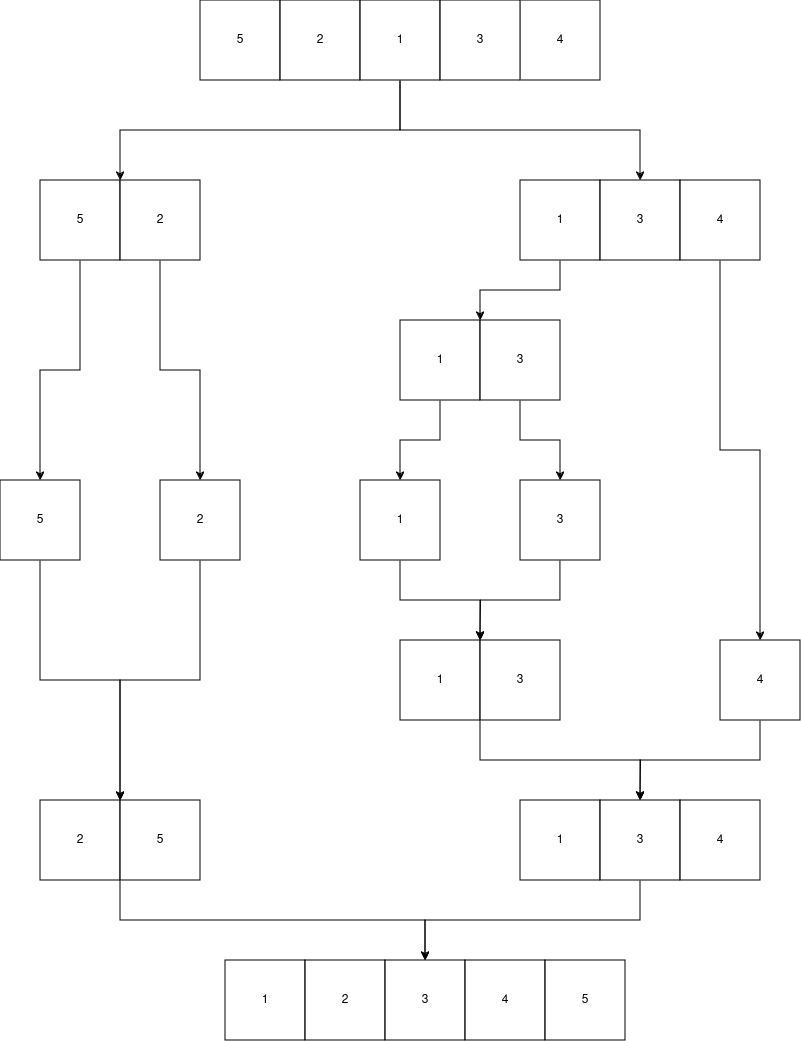
\includegraphics[width=0.7\linewidth]{images/mergesort.drawio.png}
	\caption{Reprezentacja sortowania Merge Sort}
	\label{fig:mergesort}
\end{figure}

\subsection{Git}
Kolejnym konceptem, którym zajmuje się projekt jest narzędzie git\cite{gitsite}. Pozwala ono zarządzać poszczególnymi wersjami projektów. Głównym korzeniem gita jest system commitów, czyli zapisania zmian w pliku w stosunku do commita starszego. To, w połączeniu z jego innymi możliwościami pozwala na tworzenie długich i skomplikowanych osi czasu danych projektów. 

Użycie gita można zademonstrować na prostym przykładzie. Tworzymy katalog a w nim repozytorium, uzywając komendy \texttt{git init}, jak widać na rys. \ref{fig:git_init}.

\begin{figure}[H]
	\centering
	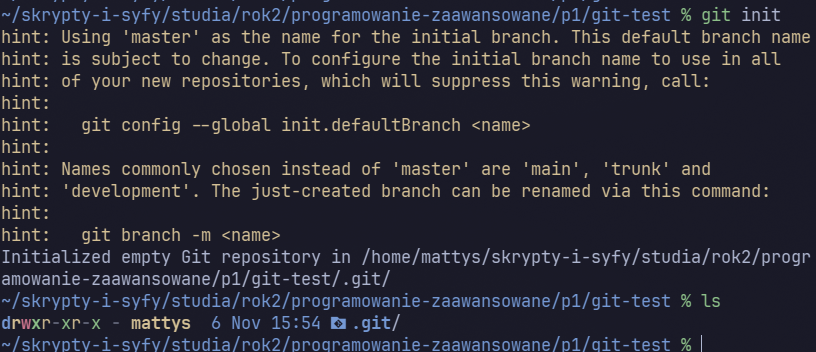
\includegraphics[width=1\textwidth]{images/git_init.png}
	\caption{\centering{Puste repozytorium git}}
	\label{fig:git_init}
\end{figure}

Stwórzmy jakiś plik i dodajmy go do repozytorium. Plik można dodać do repozytorium komendą \texttt{git add}

\begin{figure}[H]
	\centering
	
\includegraphics[width=1\textwidth]{images/git_add.png}
	\caption{\centering{Stworznie pliku w repozytorium}}
	\label{fig:git_add}
\end{figure}

Następnie należy scommitować zmiany. 

\begin{figure}[H]
	\centering
	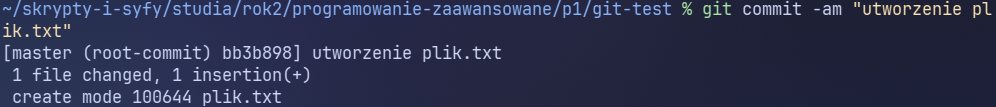
\includegraphics[width=1\textwidth]{images/git_commit1.png}
	\caption{\centering{Commit nr. 1}}
	\label{fig:git_commit1}
\end{figure}

Na rysunku \ref{fig:git_commit1} użyta komenda \texttt{git commit} commituje wszystkie dodane pliki (\texttt{-a}) z jakimś komunikatem (\texttt{-m}).  

\begin{figure}[H]
	\centering
	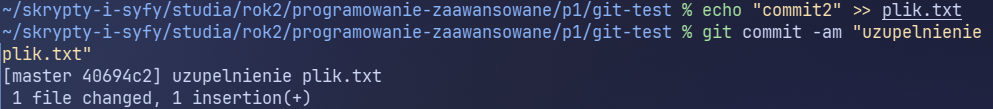
\includegraphics[width=1\textwidth]{images/git_commit2.png}
	\caption{\centering{Commit nr. 2}}
	\label{fig:git_commit2}
\end{figure}

Na rys. \ref{fig:git_commit2}, został utworzony kolejny commit, dodajacy zmiany do \texttt{plik.txt}.

\begin{figure}[H]
	\centering
	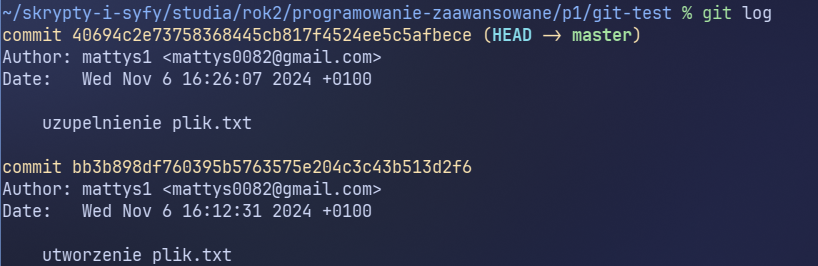
\includegraphics[width=1\textwidth]{images/git_log.png}
	\caption{\centering{Log gita}}
	\label{fig:git_log}
\end{figure}

Jak na rys. \ref{fig:git_log} jest pokazane, używając komendy \texttt{git log}, można wyświetlić log commitów w repozytorium.

\begin{figure}[H]
	\centering
	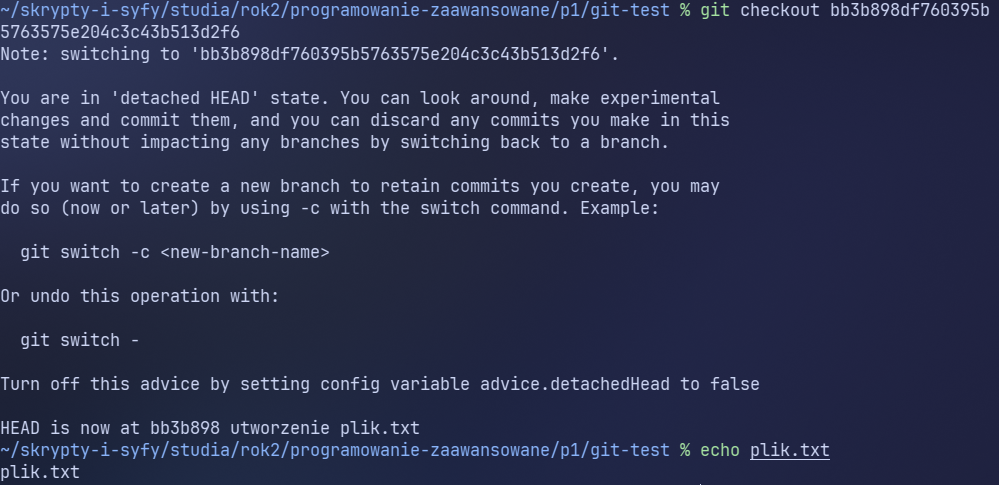
\includegraphics[width=1\textwidth]{images/git_checkout.png}
	\caption{\centering{Demonstracja checkout}}
	\label{fig:git_checkout}
\end{figure}

Jak widać na rys. \ref{fig:git_checkout}, komenda \texttt{git checkout}, pozwala na przejście repozytorium w inny stan, w tym przypadku przechodzi się do commita o danym ID, pokazanym na rys. \ref{fig:git_log}. Jako, że jest to pierwszy commit, nie ma w nim zmian z drugiego.

\subsection{Doxygen}
Doxygen\cite{doxygensite} jest narzędziem automatycznie generującym dokumentację programu z komentarzy w kodzie źródłowym. Potrafi on generować strony HTML, gdzie można dynamicznie nawigować się miedzy rożnymi częściami kodu oraz pliki \LaTeX, które można konwertować na różne, statyczne formaty.

   	\newpage
\section{Projektowanie}		%3
%Napisać z jakich narzędzi będziemy korzystać (kompilator, język programowania), git, biblioteki dodatkowe, itp.
%Opisać szczegółowe ustawienia kompilatora (jeśli są), powiązania z bibliotekami, itp.
%Narysować graf, UML, diagram klas, schemat działania algorytmu
%Jeśli zadanie zakłada przedstawienie jakiegoś narzędzia (np. git, AI) należy opisać sposób jego używania

\subsection{Implementacja Merge Sort}


Do zaimplementowania Merge Sorta zostanie użyty Język \texttt{C++} z kompilatorem \texttt{g++}. Wersja standardu \texttt{C++} to \texttt{C++20}. Jako, że projekt ma być rozdzielony na dwa pliki, zostanie zastosowany \texttt{CMake} w celu automatyzacji procesu budowania. \texttt{CMake} pozwala na generowanie plików budujących dany projekt, zgodnie z określoną konfiguracją. Oszczędza to programiście, szczególnie przy większych projektach, manualne pisanie Makefileów.
Plik konfiguracyjny \texttt{CMakeLists.txt} może wyglądać jak na rysunku

\begin{lstlisting}[caption=Plik konfiguracyjny CMake, label={lst:cmakelists}, language=C++]
	cmake_minimum_required(VERSION 3.15)
	
	set(PROJECT_NAME proj1)
	
	project(${PROJECT_NAME} VERSION 0.1 LANGUAGES CXX)
	
	set(CMAKE_CXX_STANDARD 20)
	set(CMAKE_CXX_STANDARD_REQUIRED ON)
	set(CMAKE_EXPORT_COMPILE_COMMANDS True)
	set(CMAKE_RUNTIME_OUTPUT_DIRECTORY ${CMAKE_CURRENT_LIST_DIR}/out)
	
	add_subdirectory(src)
	
\end{lstlisting}

Edytorem będzie program Neovim. Jest to terminalowy edytor tekstu z możliwością poszerzenia funkcjonalności przy użyciu wszelkiego rodzaju pluginów. Wybrany został, dlatego że jest on już skonfigurowany na moim komputerze zgodnie z moimi preferencjami.

\subsection{Git}

Dla ułatwienia pracy, zastosowany został front-end dla gita o nazwie lazygit. Jest to terminalowy program, którego główną zaletą jest łatwa nawigacja przy użyciu klawiatury. Ponadto, jest on lekki i szybki.

\subsection{Doxygen}

Konfiguracja dla Doxygena jest wygenerowana przy użyciu programu doxywizard, pokazany na rys. \ref{fig:doxywizard}, pozwalającego na graficzne zmienianie ustawień. Po wygenerowaniu konfiguracji, Doxygen wywoływany jest przy użyciu komendy.

\begin{figure}[H]
	\centering
	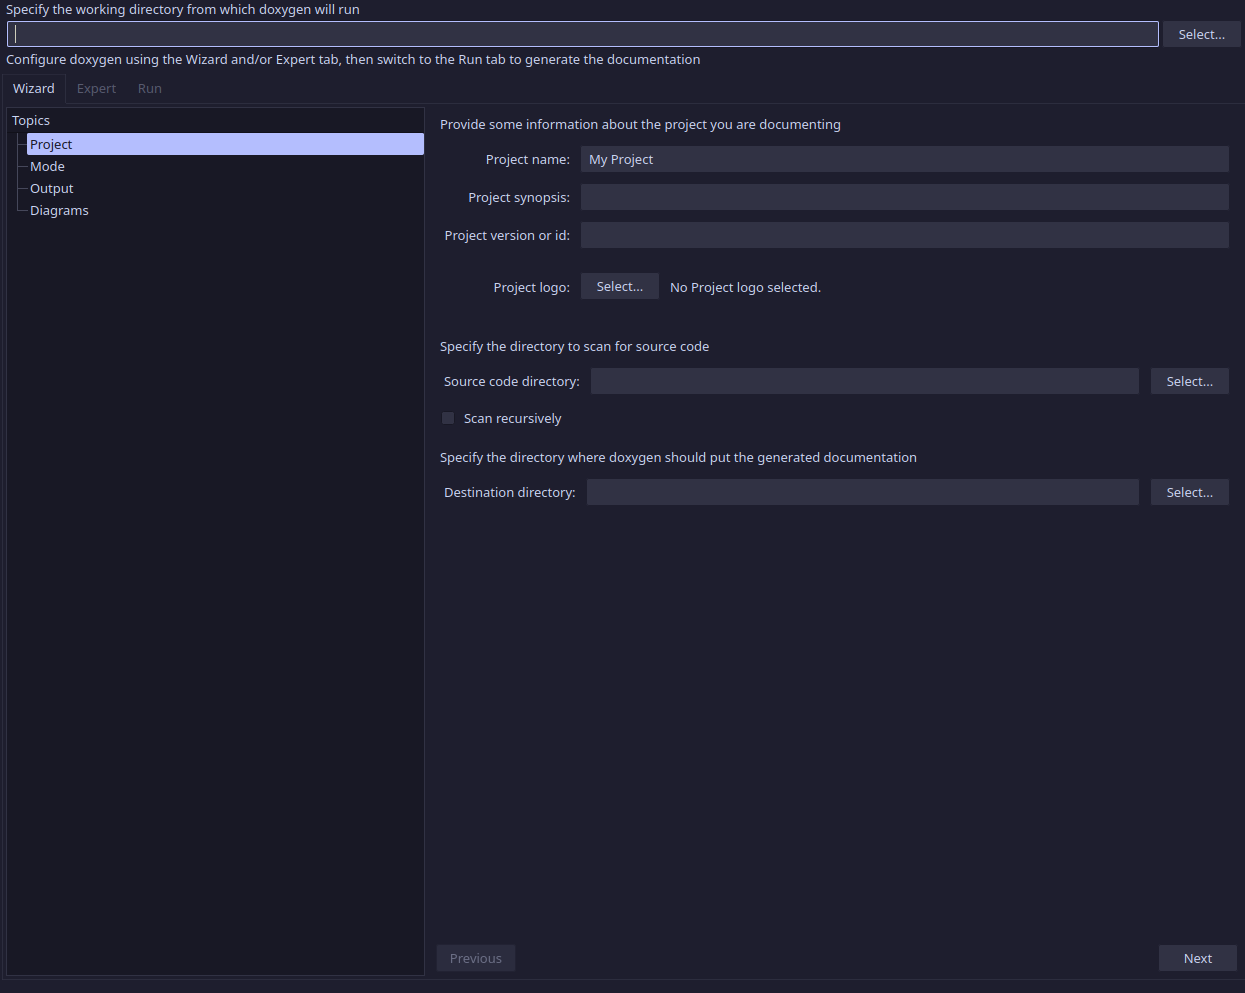
\includegraphics[width=1\textwidth]{images/doxywizard.png}
	\caption{\centering{Interfejs programu doxywizard}}
	\label{fig:doxywizard}
\end{figure}

\subsection{Google Test}

Google Test został dodany do projektu jako biblioteka w \texttt{CMake}, co zostało ukazane na listingu nr.~\ref{lst:gtestcmake}. Framework jest automatycznie pobierany i instalowany przy konfiguracji.

\begin{lstlisting}[caption=Dodanie Google Test do projektu, label={lst:gtestcmake}, language=C++]
include(FetchContent)
	FetchContent_Declare(
			googletest
			URL https://github.com/google/googletest/archive03597a01ee50ed33e9dfd640b249b4be3799d395.zip
	)
FetchContent_MakeAvailable(googletest)

\end{lstlisting}

Pliki źródłowe testów znajdują się we własnym folderze, więc też trzeba do niego dodać \texttt{CMakeLists}, jak widać na listingu nr.~\ref{lst:testscmake}

\begin{lstlisting}[caption=Dodanie Google Test do projektu, label={lst:testscmake}, language=C++]
file(GLOB_RECURSE SRC_FILES *.cpp *.h)
set(TESTS_EXECUTABLE ${PROJECT_NAME}_tests)

enable_testing()

add_executable(${TESTS_EXECUTABLE} ${SRC_FILES})

target_link_libraries(
	${TESTS_EXECUTABLE} PUBLIC
	${PROJECT_NAME}_lib
	GTest::gtest_main
)

\end{lstlisting}

Plik wykonywalny testów jest linkowany do - oprócz samego frameworka - biblioteki jaka jest wygenerowana z klasy \texttt{MergeSorter}, o której więcej w sekcji nr.~\ref{sec:MergeSorter}.

   	\newpage
\section{Implementacja}		%4
%Opisać implementacje algorytmu/programu. Pokazać ciekawe fragmenty kodu
%Opisać powstałe wyniki (algorytmu/nrzędzia)

\subsection{Ogólne informacje o implementacji klas}

\subsubsection{Klasa BSTTree}

Drzewo jest zaimplementowane jako jeden plik \texttt{.hpp}. Nie jest podzielone na plik implementacji oraz nagłówek, ponieważ jest ono szablonem. Deklaracja klasy oraz prywatne elementy wyglądają następująco:

\begin{lstlisting}[caption=Deklaracja drzewa BST, label={lst:BSTprivate}, language=C++]
	template <typename T>
	class BSTTree {
		private:
		struct Tree {
			T contents;
			Tree* parent;
			Tree* left;
			Tree* right;
			
			Tree(T _contents, Tree* _parent = nullptr, Tree* _left = nullptr, Tree* _right = nullptr):
			contents { _contents },
			parent { _parent },
			left { _left },
			right { _right } {}
			
			~Tree() {
				delete left;
				delete right;
			}
		};
		
		Tree* root;
		
		void recursive_add(const T& element, Tree*& node, Tree* parentNode = nullptr) {
			if(node == nullptr) {
				node = new Tree(element);
				
				if(parentNode == nullptr) {
					return;
				}
				
				node->parent = parentNode;
				
				if(node->contents >= parentNode->contents) {
					parentNode->right = node;
				} else {
					parentNode->left = node;
				}
				
				return;
			}
			
			if(element >= node->contents) {
				recursive_add(element, node->right, node);
			} else {
				recursive_add(element, node->left, node);
			}	
		}
		
		void preorder_traverse_recursive(Tree* node, std::vector<Tree*>& traversedTrees) {
			if(node == nullptr) {
				return;
			}
			
			traversedTrees.push_back(node);
			
			preorder_traverse_recursive(node->left, traversedTrees);
			preorder_traverse_recursive(node->right, traversedTrees);
		}
		
		void inorder_traverse_recursive(Tree* node, std::vector<Tree*>& traversedTrees) {
			if(node == nullptr) {
				return;
			}
			
			inorder_traverse_recursive(node->left, traversedTrees);
			
			traversedTrees.push_back(node);
			
			inorder_traverse_recursive(node->right, traversedTrees);
		}
		
		void postorder_traverse_recursive(Tree* node, std::vector<Tree*>& traversedTrees) {
			if(node == nullptr) {
				return;
			}
			
			postorder_traverse_recursive(node->left, traversedTrees);
			postorder_traverse_recursive(node->right, traversedTrees);
			
			traversedTrees.push_back(node);
		}
		public:
			...
\end{lstlisting}

Jak widać w kodzie zamieszczonym na listingu nr \ref{lst:BSTprivate}., Klasa jest wrapperem dla structa \texttt{Tree}, zadeklarowanego na linijce nr. 4. Struct ten ma trzy wskaźniki - \texttt{left} dla elementu lewego, \texttt{right} dla elementu prawego, \texttt{parent} dla elementu będącego rodzicem oraz zawartość \texttt{contents}, opsującą element zawarty w danym węźle. 

W linii 10 zadeklarowany jest konstruktor, który domyślnie ustawia wartości wskaźników rodzica, dziecka lewego oraz prawego na \texttt{nullptr}. Istnieje możliwość sprecyzowania wartości wskaźników.

Od linii 16 do 18 znajduje się destruktor drzewa. W destruktorze węzeł lewy i prawy jest usuwany.

Od linijki nr 24, do końca fragmentu, zawarty jest szereg pomocniczych metod prywatnych. Ich działanie zostanie omówione przy dyskusji korzystających z nich metod publicznych.

Jedną z tych metod publicznych jest \texttt{add()}, którą widać na listingu nr \ref{lst:BSTadd}

\begin{lstlisting}[caption=Metoda \texttt{add()}, label={lst:BSTadd}, language=C++]
	void add(const T& element) {
		recursive_add(element, root);
	}

\end{lstlisting}

Metoda ta przyjmuje parametr \texttt{element}, który będzie wartością nowo dodanego węzła. W swoim ciele, wywołuje ona prywatną metodę \texttt{recursive\_add()} z parametrami \texttt{element} i korzeniem drzewa \texttt{root}. Jej definicja jest zawarta w linijce 24, listingu nr \ref{lst:BSTprivate}. 

Metoda \texttt{recursive\_add()} działa na zasadzie rekurencji. Na początku funkcji sprawdzane jest czy teraźniejszy \texttt{node} to \texttt{nullptr}. Jeżeli tak, oznacza to, że doszło się do końca drzewa i można ten wskaźnik ustawić jako nowy węzeł. Na linijce nr. 28, sprawdzane jest czy rodzic wskaźnika \texttt{node} to \texttt{nullptr}. Jeżeli tak, oznaczałoby to, że pracujemy ze wskaźnikiem \texttt{root}. Wracamy wtedy wcześnie z funkcji, dlatego że \texttt{root} nie ma rodzica, więc nie chcemy manipulować wskaźnikami tego rodzica. Następnie, po zakończeniu bloku \texttt{if}, ustawiane są wskaźniki rodzica. Na linijce nr. 43, metoda wywoływana jest ponownie, w zależności od tego czy zawartość \texttt{node} jest większa od liczby która ma być dodana, czy nie.

Kolejną metodą na jaką można zwrócić uwagę to \texttt{traverse\_preorder()}, zawarta na listingu nr \ref{lst:BSTtraverse_preorder}. 

\begin{lstlisting}[caption=Metoda \texttt{add()}, label={lst:BSTtraverse_preorder}, language=C++]
	std::vector<T> traverse_preorder(void) {
		std::vector<Tree*> traversedTrees;
	
		preorder_traverse_recursive(root, traversedTrees);

		return traversedTrees 
		| std::ranges::views::transform(
				[](const Tree* tree) { return tree->contents; }
		) 
		| std::ranges::to<std::vector>(); 
	}

\end{lstlisting}

Metoda \texttt{traverse\_preorder()}, ma za zadanie zwrócić wektor wartości węzłów ułożonych w kolejności preorder drzewa. Ku temu celu, na początku metody, w linijce nr 2 listingu nr \ref{lst:BSTtraverse_preorder}, deklarowany jest wektor \texttt{traversedTrees}, który będzie wypełniony wskaźnikami \texttt{Tree*} w kolejności preorder. Do wypełnienia tego wektora, używana jest prywatna metoda \texttt{preorder\_traverse\_recursive()} z parametrami \texttt{root} i \texttt{traversedTrees}.

Metoda \texttt{preorder\_traverse\_recursive()}, podobnie jak inne prywatne metody jest zawarta na listingu nr \ref{lst:BSTprivate}, konkretnie od linijki nr. 50 do linijki nr. 59. Na początku metody, sprawdzane jest czy parametr \texttt{node} jest równy \texttt{nullptr} - oznaczałoby to, że dotarło się do końca danej ścieżki w drzewie i należy się wrócić. Następnie bieżący \texttt{node} jest pushowany do wektora \texttt{traversedTrees}, po czym w linijkach nr. 57 i 58, wywoływana jest dwukrotnie metoda \texttt{preorder\_traverse\_recursive()}. Za pierwszym razem na lewy, węzeł, a za drugim na prawym. Takie wywołanie sprawi, że najpierw odwiedzone zostaną lewe gałęzie, a dopiero później prawe, zgodnie z porządkiem preorder.

Wracając z metody \texttt{preorder\_traverse\_recursive()} do metody \texttt{traverse\_preorder()} i listingu nr \ref{lst:BSTtraverse_preorder}, w linijce nr. 6, widać że do \texttt{traversedTrees} aplikowana jest transformacja przy użyciu biblioteki \texttt{std::ranges}, powodująca, że zwrócony zostanie wektor zawartości poszczególnych węzłów.

\subsubsection{Klasa FileTree} 

Głównym zadaniem klasy FileTree jest odczyt i zapis zawartość drzewa z, jak i do pliku. Odbywa się to na dwa sposoby: 1 - do zwykłego pliku tekstowego(.txt) oraz 2 - do pliku binarnego(.bin). Klasa zawiera 4 metody publiczne:
\begin{itemize}
	\item save\_to\_text() - Ta metoda odpowiedzialna jest za zapisywanie zawartości drzewa binarnego do pliku tekstowego.
	\item load\_from\_file() - Ta metoda odpowiedzialna jest za wczytywanie zawartości pliku tekstowego do drzewa binarnego.
	\item analogicznie działają metody do drzewa binarnego.
\end{itemize}

Na listingu nr \ref{lst:FileTree-class} przedstawiona jest klasa FileTree.
\begin{lstlisting}[caption=Klasa \texttt{FileTree}, label={lst:FileTree-class}, language=C++]
	
	template <typename T>
	class FileTree {
		public:
		void save_to_text(const std::string& filename, const std::vector<T>& elements) {
			std::ofstream file(filename);
			if (!file) {
				std::cerr << "Error: Could not open file for writing.\n";
				return;
			}
			for (const auto& elem : elements) {
				file << elem << " ";
			}
		}
		void load_from_text(const std::string& filename, BSTTree<T>& tree, std::vector<T>& elements, bool append = false) {
			std::ifstream file(filename);
			if (!file) {
				std::cerr << "Error: Could not open file for reading.\n";
				return;
			}
			if (!append) {
				tree.delete_tree();
				elements.clear();
			}
			T value;
			while (file >> value) {
				elements.push_back(value);
				tree.add(value);
			}
		}
		void save_to_binary(const std::string& filename, const std::vector<T>& elements) {
			std::ofstream file(filename, std::ios::binary);
			if (!file) {
				std::cerr << "Error: Could not open file for binary writing.\n";
				return;
			}
			size_t size = elements.size();
			file.write(reinterpret_cast<const char*>(&size), sizeof(size));
			for (const auto& elem : elements) {
				file.write(reinterpret_cast<const char*>(&elem), sizeof(T));
			}
		}
		void load_from_binary(const std::string& filename, BSTTree<T>& tree, std::vector<T>& elements, bool append = false) {
			std::ifstream file(filename, std::ios::binary);
			if (!file) {
				std::cerr << "Error: Could not open file for binary reading.\n";
				return;
			}
			if (!append) {
				tree.delete_tree();
				elements.clear();
			}
			size_t size = 0;
			file.read(reinterpret_cast<char*>(&size), sizeof(size));
			for (size_t i = 0; i < size; ++i) {
				T elem;
				file.read(reinterpret_cast<char*>(&elem), sizeof(T));
				elements.push_back(elem);
				tree.add(elem);
			}
		}
	};
\end{lstlisting}
jak widać na listingu, klasa nie posiada żadnych metod prywatnych.
Klasa składa się z 4 metod publicznych, zadeklarowanych w wiersach: 5, 15, 31, 43. Poniżej dokładniejsze objaśnienie działania metod.

\begin{lstlisting}[caption=Metoda \texttt{save\_to\_file}, label={lst:FileTree-savetext}, language=C++]
	void save_to_text(const std::string& filename, const std::vector<T>& elements) {
		std::ofstream file(filename);
		if (!file) {
			std::cerr << "Error: Could not open file for writing.\n";
			return;
		}
		for (const auto& elem : elements) {
			file << elem << " ";
		}
	}
\end{lstlisting}

Jak widać na listingu nr \ref{lst:FileTree-savetext} metoda ma dwa parametry: filename - które definiuje nazwę pliku do którego zostanie zapisana zawartość tablicy oraz elements - który jest wektorem elementów które zostaną zapisane do pliku. Polecenie w wierszu 2 otwiera plik, jeżeli nie istnieje jest tworzony.
Następnie w wierszu 3 mamy instrukcję if. Jeżeli plik nie może być otwarty wysyłany jest komunikat o błędzie. Jeżeli plik się otworzy, to w wierszu 7 zadeklarowana jest pętla która iteruje przez wszystkie elementy drzewa binarnego patrząc na kolejność ich dodania oraz dodaje je do pliku poleceniem w wierszu 8.


\begin{lstlisting}[caption=Metoda \texttt{load\_to\_file}, label={lst:FileTree-loadtext}, language=C++]
	void load_from_text(const std::string& filename, BSTTree<T>& tree, std::vector<T>& elements, bool append = false) {
		std::ifstream file(filename);
		if (!file) {
			std::cerr << "Error: Could not open file for reading.\n";
			return;
		}
		if (!append) {
			tree.delete_tree();
			elements.clear();
		}
		T value;
		while (file >> value) {
			elements.push_back(value);
			tree.add(value);
		}
	}
\end{lstlisting}

Na listingu nr \ref{lst:FileTree-loadtext} przedstawiona jest metoda wczytywania danych z pliku tekstowego do drzewa binarnego. Metoda zawiera 4 parametry: filename - nazwa pliku, tree - drzewo binarne do którego będą dodane będą wartości, elements - wketor przechowujący wartości do dodania oraz append - który polega na kontroli dodawania wartości do już istniejącego drzewa z wartościami. Append jest ustawiony na false dlatego drzewo będzie czyszczone oraz następne wartości zostaną dodane do drzewa.

W wierszu 2 przedstawiona jest instrukcja wyświetlenia komunikatu błędu w przypadku gdy pliku nie da się otworzyć.

W wierszach 7, 8 i 9 przedstawiona jest seria instrukcji odpowiedzialna za czyszczenie drzewa binarnego z poprzednich wartości.

W wierszach 11, 12, 13 oraz 14 przedstawiona jest pętla while która dodaje wartości do tablicy w takiej samej kolejności w jakiej są zapisane w pliku tekstowym.

\begin{lstlisting}[caption=Metoda \texttt{save\_to\_binary}, label={lst:FileTree-savebinary}, language=C++]
	void save_to_binary(const std::string& filename, const std::vector<T>& elements) {
		std::ofstream file(filename, std::ios::binary);
		if (!file) {
			std::cerr << "Error: Could not open file for binary writing.\n";
			return;
		}
		size_t size = elements.size();
		file.write(reinterpret_cast<const char*>(&size), sizeof(size));
		for (const auto& elem : elements) {
			file.write(reinterpret_cast<const char*>(&elem), sizeof(T));
		}
	}
\end{lstlisting}
Na listingu \ref{lst:FileTree-savebinary} przedstawiona jest metoda zapisu danych z drzewa do pliku binarnego. Metoda posiada 2 parametry: filename - nazwa pliku oraz elements - wektor elementów do zapisania.

W wierszu 2 znajduje się instrukcja tworząca plik binarny, aby stworzyć taki plik trzeba zastosować "std::ios::binary".

W wierszach 3 i 4 znajduje się instrukcja if która wyświetli komunikat o błędzie w przypadku gdy pliku nie uda się otworzyć.

W wierszach od 7 do 11 znajduje się szereg instrukcji odpowiedzialnych za zapis danych z drzewa do pliku binarnego.

Polecenie w wierszu 7 odpowiedzialne jest za ustalenie liczby elementów w wektorze.
Polecenie w wierszu 8 zapisuje bity z pamięci do pliku za pomocą "file.write()". Polecenie "reinterpret\_cast<const char*> jest odpowiedzialne za konwersję adresu size na wskaźnik const char*, jest to wymagane ponieważ write zapisuje bity bezpośrednio z pamięci. sizeof() definiuje ile bitów należy zapisać.

Następnie za pomocą pętli for w wierszu 9, 10 oraz 11 każdy element zapisywany jest do pliku binarnego.

\begin{lstlisting}[caption=Metoda \texttt{load\_to\_binary}, label={lst:FileTree-loadbinary}, language=C++]
	void load_from_binary(const std::string& filename, BSTTree<T>& tree, std::vector<T>& elements, bool append = false) {
		std::ifstream file(filename, std::ios::binary);
		if (!file) {
			std::cerr << "Error: Could not open file for binary reading.\n";
			return;
		}
		if (!append) {
			tree.delete_tree();
			elements.clear();
		}
		size_t size = 0;
		file.read(reinterpret_cast<char*>(&size), sizeof(size));
		for (size_t i = 0; i < size; ++i) {
			T elem;
			file.read(reinterpret_cast<char*>(&elem), sizeof(T));
			elements.push_back(elem);
			tree.add(elem);
		}
	}
\end{lstlisting}
Na listingu \ref{lst:FileTree-loadbinary} przedstawiona jest metoda wczytywania elementów z pliku binarnego do drzewa binarnego.
Metoda zawiera 4 parametry: filename - nazwa pliku, tree - wskazujące na drzewo do którego zostaną wczytane wartości, elements - wektor przechowujący elementy do wczytania oraz append - decydujący o dodaniu wartości z drzewa binarnego do istniejącej tablicy lub nie.

W wierszu 2 otwierany jest plik binarny poleceniem "std::ifstream()".
Instrukcja if w wierszach od 3 do 6 odpowiedzialna jest za wyświetlenie komunikatu o błędzie w przypadku gdy pliku nie uda się otworzyć.
Instrukcja if w wiersach od 7 do 10 odpowiedzialna jest za czyszczenie drzewa z poprzednich wartości przed dodaniem nowych.
Dodawanie wartości do drzewa binarnego odbywa się w wierszach od 11 do 18.
W wierszu 11 oraz 12 czytana jest część pliku bin przechowująca liczbę przechowywanych elementów. "reinterpret\_cast<char*>(...) odpowiedzialne jest za konwersję bitów na postać bardziej odpowiednią do odczytu. sizeof(...) odpowiedzialne jest za liczbę bitów do odczytania.
Następnie w wierszach od 13 do 18 sczytywane są wszystkie wartości oraz dodawane do drzewa. Polecenie w wierszu 16 sprawdza jest odpowiedzialne za dodawanie elementów w takiej samej kolejności w jakiej są zapisane na pliku bin. Polecenie w wierszu 17 dodaje elementy.

\subsubsection{Klasa main}
\begin{lstlisting}[caption=Klasa \texttt{main}, label={lst:main-class}, language=C++]
	int main(int argc, char* argv[]) {
		BSTTree<int> tree;
		BSTTree<int> tree2;
		FileTree<int> fileTree;
		std::vector<int> elements;
		
		int option;
		int option2;
		int value;
		std::println("List of options:");
		std::println("1 - add element | 2 - remove element | 3 - print traversal preordern");
		std::println("4 - print traversal inorder | 5 - print traversal postorder | 6 - export to file");
		std::println("7 - import from file | 8 - delete tree | 9 - fid path to element");
		std::println();
		do {
			std::print("What do you want to do? "), std::cin >> option;
			
			switch (option) {
				case 1:
				std::print("Insert element to add: ");
				std::cin >> value;
				tree.add(value);
				elements.push_back(value);
				break;
				
				case 2:
				std::print("Insert element to remove: ");
				std::cin >> value;
				tree.delete_element(value);
				break;
				
				case 3:
				std::print("Preorder traversal:\n");
				for (const auto& item : tree.traverse_preorder()) {
					std::print("{}, ", item);
				}
				std::print("\n");
				break;
				
				case 4:
				std::print("Inorder traversal:\n");
				for (const auto& item : tree.traverse_inorder()) {
					std::print("{}, ", item);
				}
				std::print("\n");
				break;
				
				case 5:
				std::print("Postorder traversal:\n");
				for (const auto& item : tree.traverse_postorder()) {
					std::print("{}, ", item);
				}
				std::print("\n");
				break;
				
				case 6:
				std::print("1 - To text | 2 - To binary\n");
				std::print("Do you want to export to text or binary file? ");
				std::cin >> option2;
				if (option2 == 1) {
					fileTree.save_to_text("tree.txt", elements);
					std::print("Tree saved to text file.\n");
				}
				else if (option2 == 2) {
					fileTree.save_to_binary("tree.bin", elements);
					std::print("Tree saved to binary file.\n");
				}
				break;
				
				case 7:
				std::print("1 - From text | 2 - From binary\n");
				std::print("Do you want to import from text or binary file? ");
				std::cin >> option2;
				if (option2 == 1) {
					fileTree.load_from_text("tree.txt", tree, elements);
					std::print("Tree loaded from text file.\n");
				}
				else if (option2 == 2) {
					fileTree.load_from_binary("tree.bin", tree, elements);
					std::print("Tree loaded from binary file.\n");
				}
				break;
				case 8:
				tree.delete_tree();
				std::print("Tree deleted.\n");
				break;
				
				case 9: {
					std::print("Input the value to search: "), std::cin >> value;
					auto path = tree.find_path(value);
					if (path.empty()) {
						std::print("Element not found.\n");
					}
					else {
						std::print("Path: ");
						for (const auto& item : path) {
							std::print("{} ", item);
						}
						std::print("\n");
					}
				}
				break;
				
				
				default:
				std::print("Invalid option. Try again.\n");
				break;
			}
		} while (lauf());
		
		return 0;
	}
\end{lstlisting}
Na listingu nr \ref{lst:main-class} przedstawiona jest klasa main. Klasa main odpowiedzialna jest za sterowaniem operacjami na drzewie binarnym. Do przeprowadzania operacji stworzone zostało menu, które podgląd wyboru dostępnych opcji oraz prośbę o wybranie opcji działania.
Następnie, w zależności od wyboru opcji instrukcja switch wywołuje odpowiednią metodę z klasy \texttt{BSTTree}.
Po wykonaniu operacji wyświetlany jest komunikat o kontynuacji lub zakończeniu działania programu. Wykorzystywana jest do tego funkcja "bool lauf" przedstawiona na listingu nr \ref{lst:main-lauf}
\begin{lstlisting}[caption=Funkcja \texttt{lauf()}, label={lst:main-lauf}, language=C++]
	bool lauf()
	{
		std::string input;
		std::cout << "\nDo you want to repeat? (type yes ocontinue, no to stop): ", std::cin >> input;
		do {
			if (input == "Yes" || input == "yes" || input== "y") {
				return true;
			}
			else if (input == "no" || input == "No" || input == "n") {
				return false;
			}
			else {
				std::cout << "insert ONLY yes or no", std::cin >> input;
			}
		} while (true);
\end{lstlisting}
Funkcja jest odpowiedzialna za sprawdzanie czy podano poprawną wartość w komunikacje o kontynuacji lub zakończeniu programu.

\subsection{Ciekawe fragmenty kodu}

\begin{lstlisting}[caption=Metoda \texttt{delete\_element()}, label={lst:delete_element_excerpt}, language=C++]
	int delete_element(T value) {
	...
		if (elementOfValue->left == nullptr && elementOfValue->right == nullptr) {
			if (elementOfValue->parent != nullptr) {
				if(elementOfValue->parent->left == elementOfValue) {
					elementOfValue->parent->left = nullptr;
				} else {
					elementOfValue->parent->right = nullptr;
				}
			}

			delete elementOfValue;
		} else {
	...
	}
\end{lstlisting}

Na listingu nr. \ref{lst:delete_element_excerpt}, widać od linijki nr. 3 zanestowane zdania \texttt{if}. Służą one do sprawdzania, czy dziecko \texttt{elementOfValue} jest połączone z rodzicem od lewej czy prawej strony, po czym wskaźnik rodzica jest zmieniany na \texttt{nullptr}. Dlatego, że C++ nie posiada łatwej możliwości tworzenia referencji do wskaźników, np. przy użyciu operatora \texttt{?}, czy lambdy, należy użyć takich niezbyt ładnych zabiegów.

   	\newpage
\section{Wnioski}	%5
%Npisać wnioski końcowe z przeprowadzonego projektu, 

\begin{itemize}
	\item Konstrukcja drzewa binarnego przydaje się wtedy, kiedy mamy zamiar kilkakrotnie wyszukiwać dane z nieposortowanego zbioru
	
	\item Branchowanie w git bardzo pomaga w pracy kolaboracyjnej
	
	\item Rekurencja w pewnych algorytmach jest prostszym rozwiązaniem do zaimplementowania niż metody iteracyjne
\end{itemize}


   
       
%%%%%%%%%%%%%%%%%%% koniec treść główna dokumentu %%%%%%%%%%%%%%%%%%%%%
	\newpage
    \addcontentsline{toc}{section}{Literatura}  
	\printbibliography

    \newpage
    \hypersetup{linkcolor=black}
    \renewcommand{\cftparskip}{3pt}
    \clearpage
    \renewcommand{\cftloftitlefont}{\Large\bfseries\sffamily}
    \listoffigures
    \addcontentsline{toc}{section}{Spis rysunków}
	\thispagestyle{fancy}
	
    \newpage
    \renewcommand{\cftlottitlefont}{\Large\bfseries\sffamily}
    \def\listtablename{Spis tabel}
    \addcontentsline{toc}{section}{Spis tabel}\listoftables 
	\thispagestyle{fancy}
	
	\newpage
	\renewcommand{\cftlottitlefont}{\Large\bfseries\sffamily}
	\renewcommand\lstlistlistingname{Spis listingów}
	\addcontentsline{toc}{section}{Spis listingów}\lstlistoflistings 
	\thispagestyle{fancy}
	


    %lista rzeczy do zrobienia: wypisuje na koñcu dokumentu, patrz: pakiet todo.sty
    \todos
    %koniec listy rzeczy do zrobienia
\end{document}
